\subsection{Zigbee2MQTT}
Um das Offizielle Zigbee2MQTT Home Assistant Add-on nutzen zu können müssen wir zunächst im Supervisor Add-on Shop(vgl. Abb, \ref{fig:ha14}: \nameref{fig:ha14}) das Repository\footnote{GITHUB: \url{https://github.com/zigbee2mqtt/hassio-zigbee2mqtt}} hinzufügen. Hierdurch erhalten wir die möglichkeit das Add-on auf unserem Home Assistant zNachdem das Geschehen ist können wir das Add-on Zigbee2MQTT installieren und starten. An diesem Punkt starten wir das System neu um alle neu installierten Erweiterungen neu zu laden.
Um eine Korrekte Konfiguration zu ermöglichen öffnen wir innerhalb des Zigbee2MQTT Add-on's den Reiter Konfiguration. Hier sehen wir die Inhalte der configuration.yaml Datei (vgl. Anhang \ref{ah_yaml_ha_configuration}: \nameref{ah_yaml_ha_configuration})

\begin{figure}[H]
    \begin{subfigure}{.5\linewidth}
        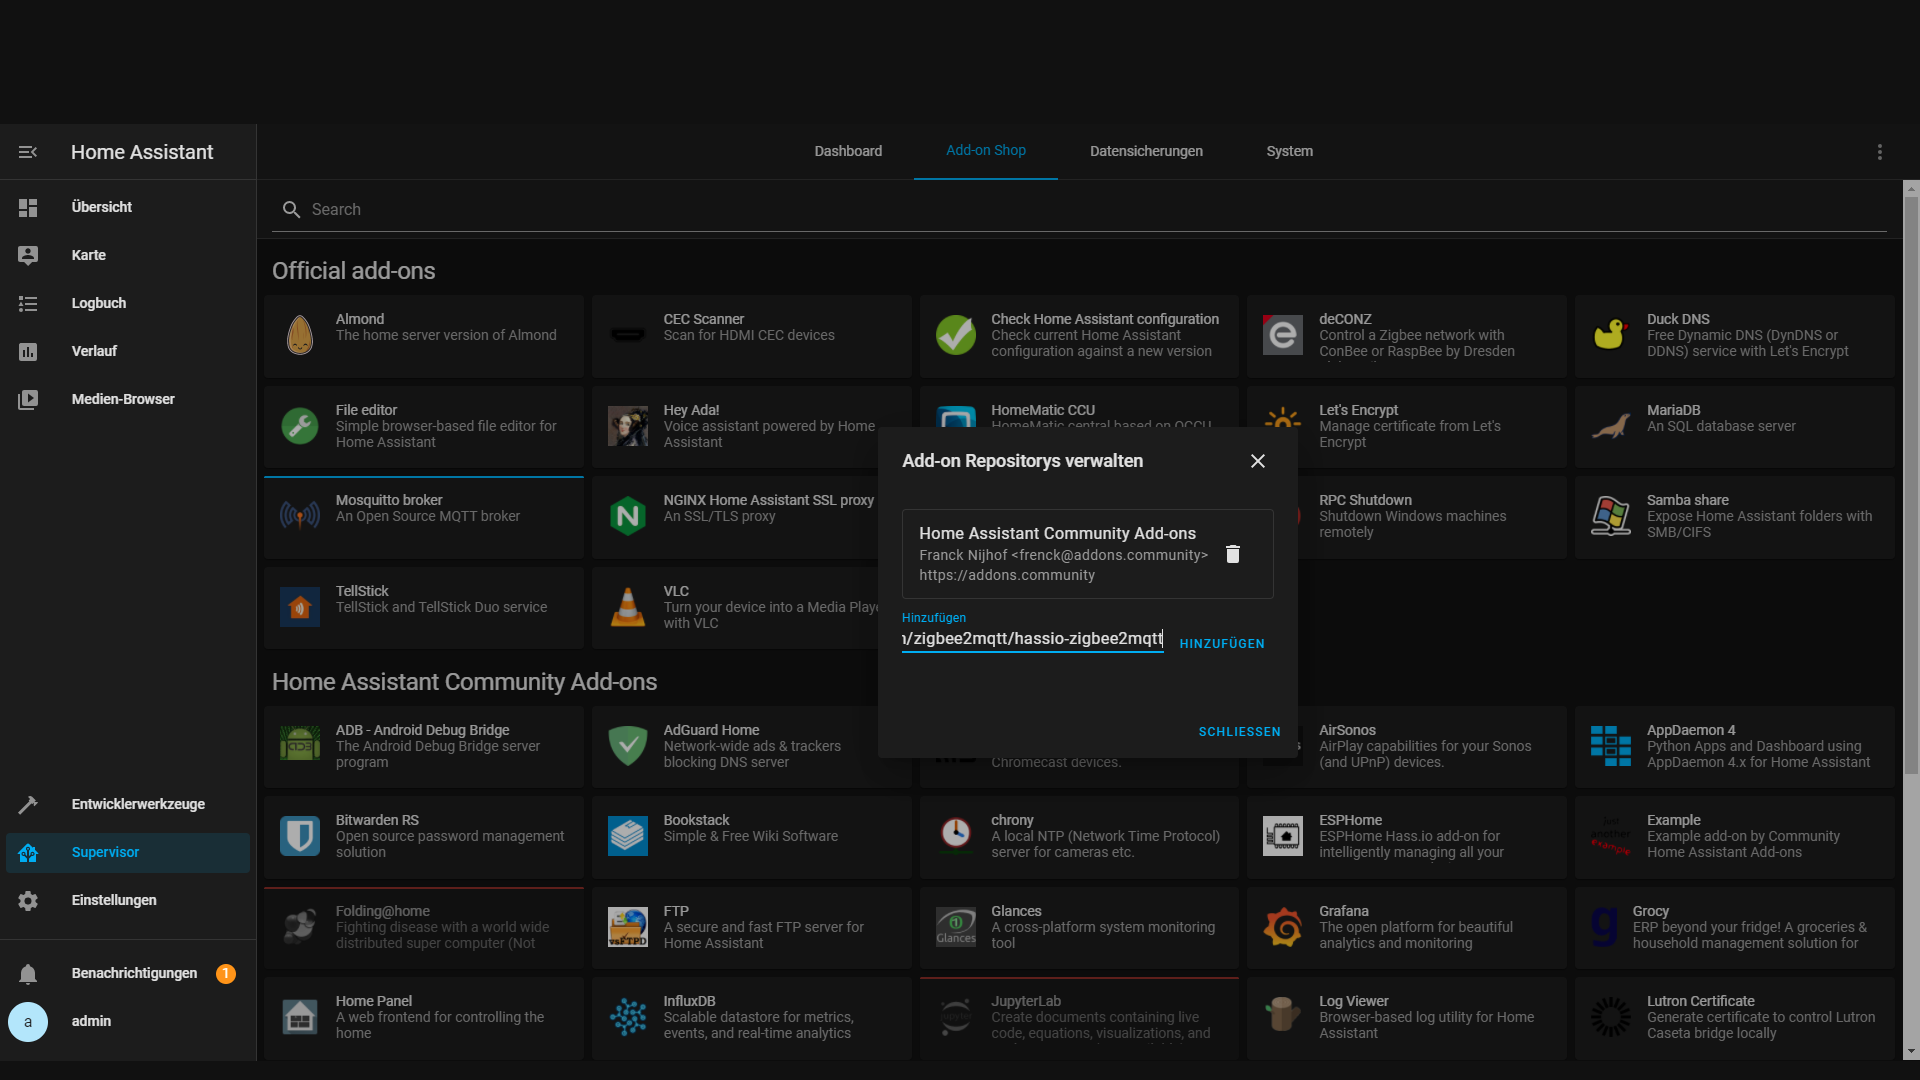
\includegraphics[width=1\textwidth]{img/HA18.png}
        \caption{Repository in Add-on Shop einpflegen}
        \label{fig:ha14}
    \end{subfigure}
%    \begin{subfigure}{.5\linewidth}
%        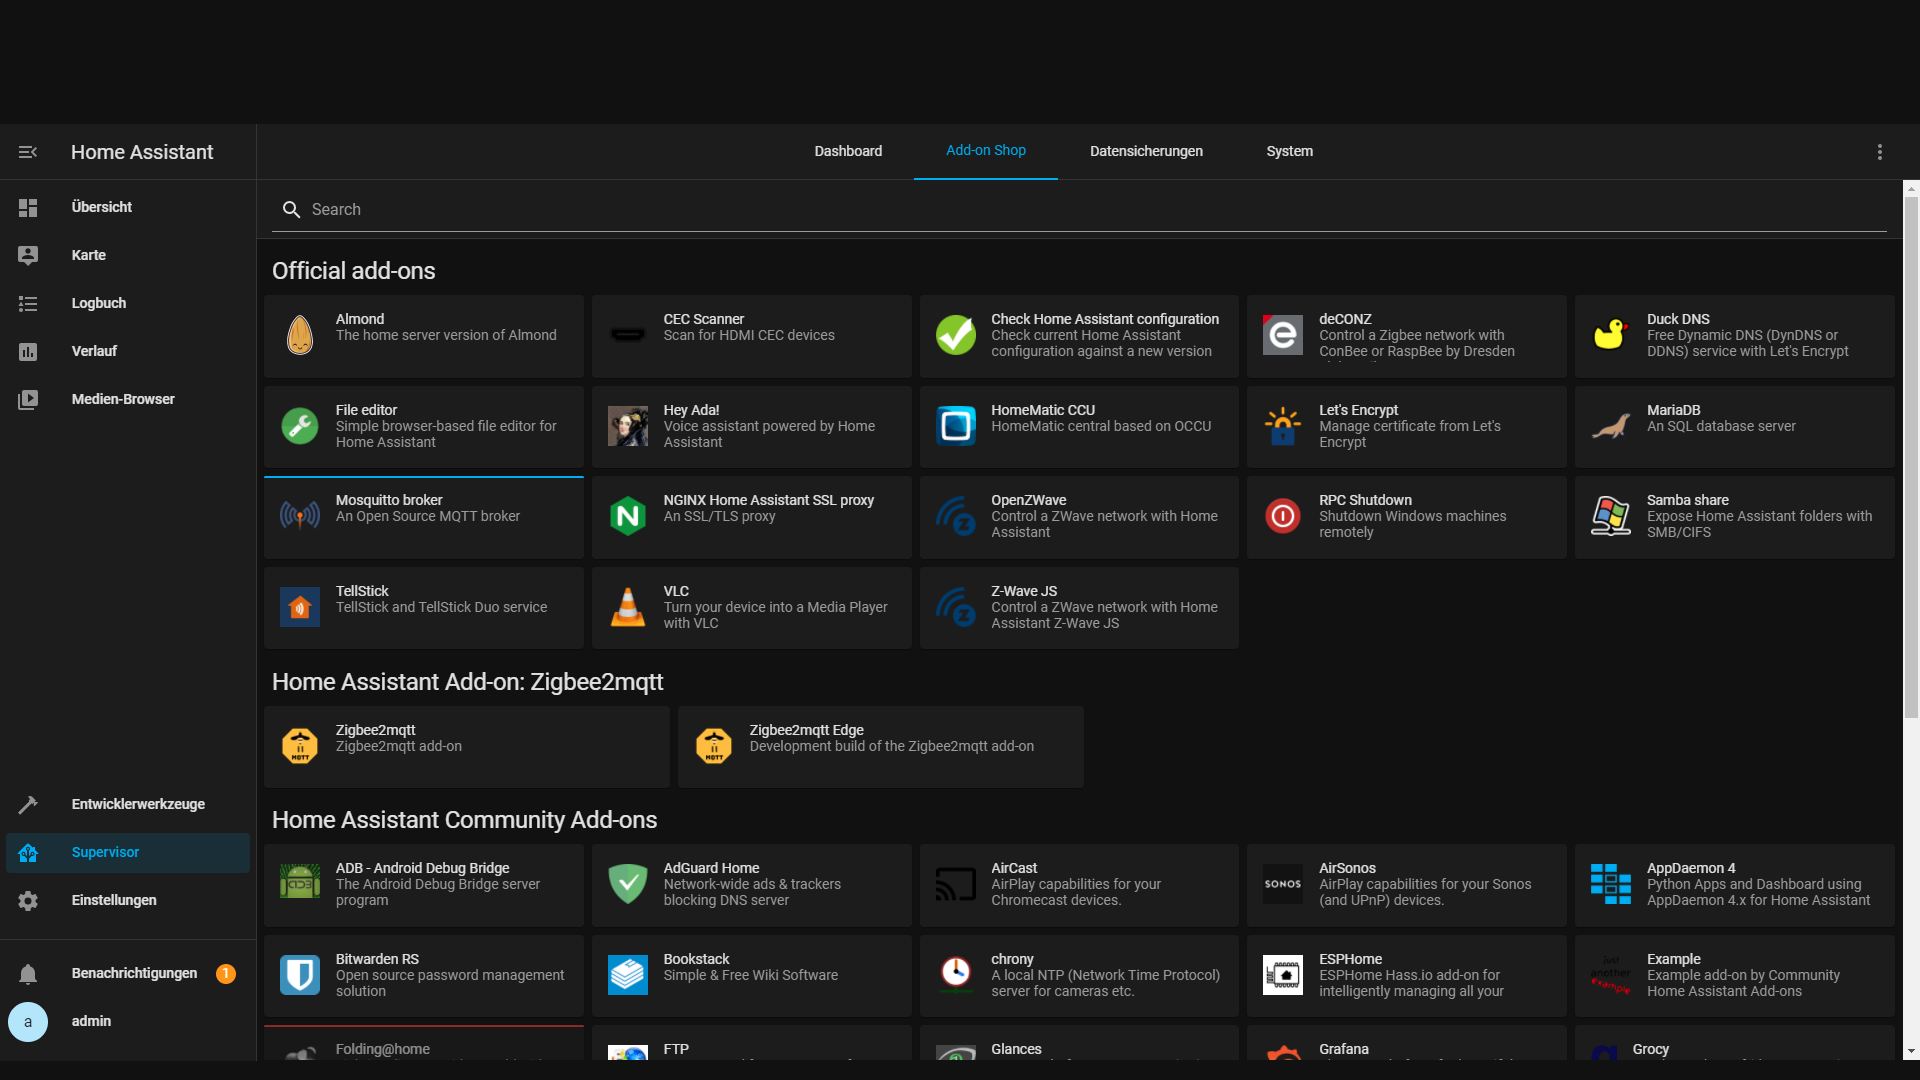
\includegraphics[width=1\textwidth]{img/HA19.png}
%        \caption{Supervisor Add-on Shop}
%        \label{fig:ha15}
%    \end{subfigure}
    \begin{subfigure}{.5\linewidth}
        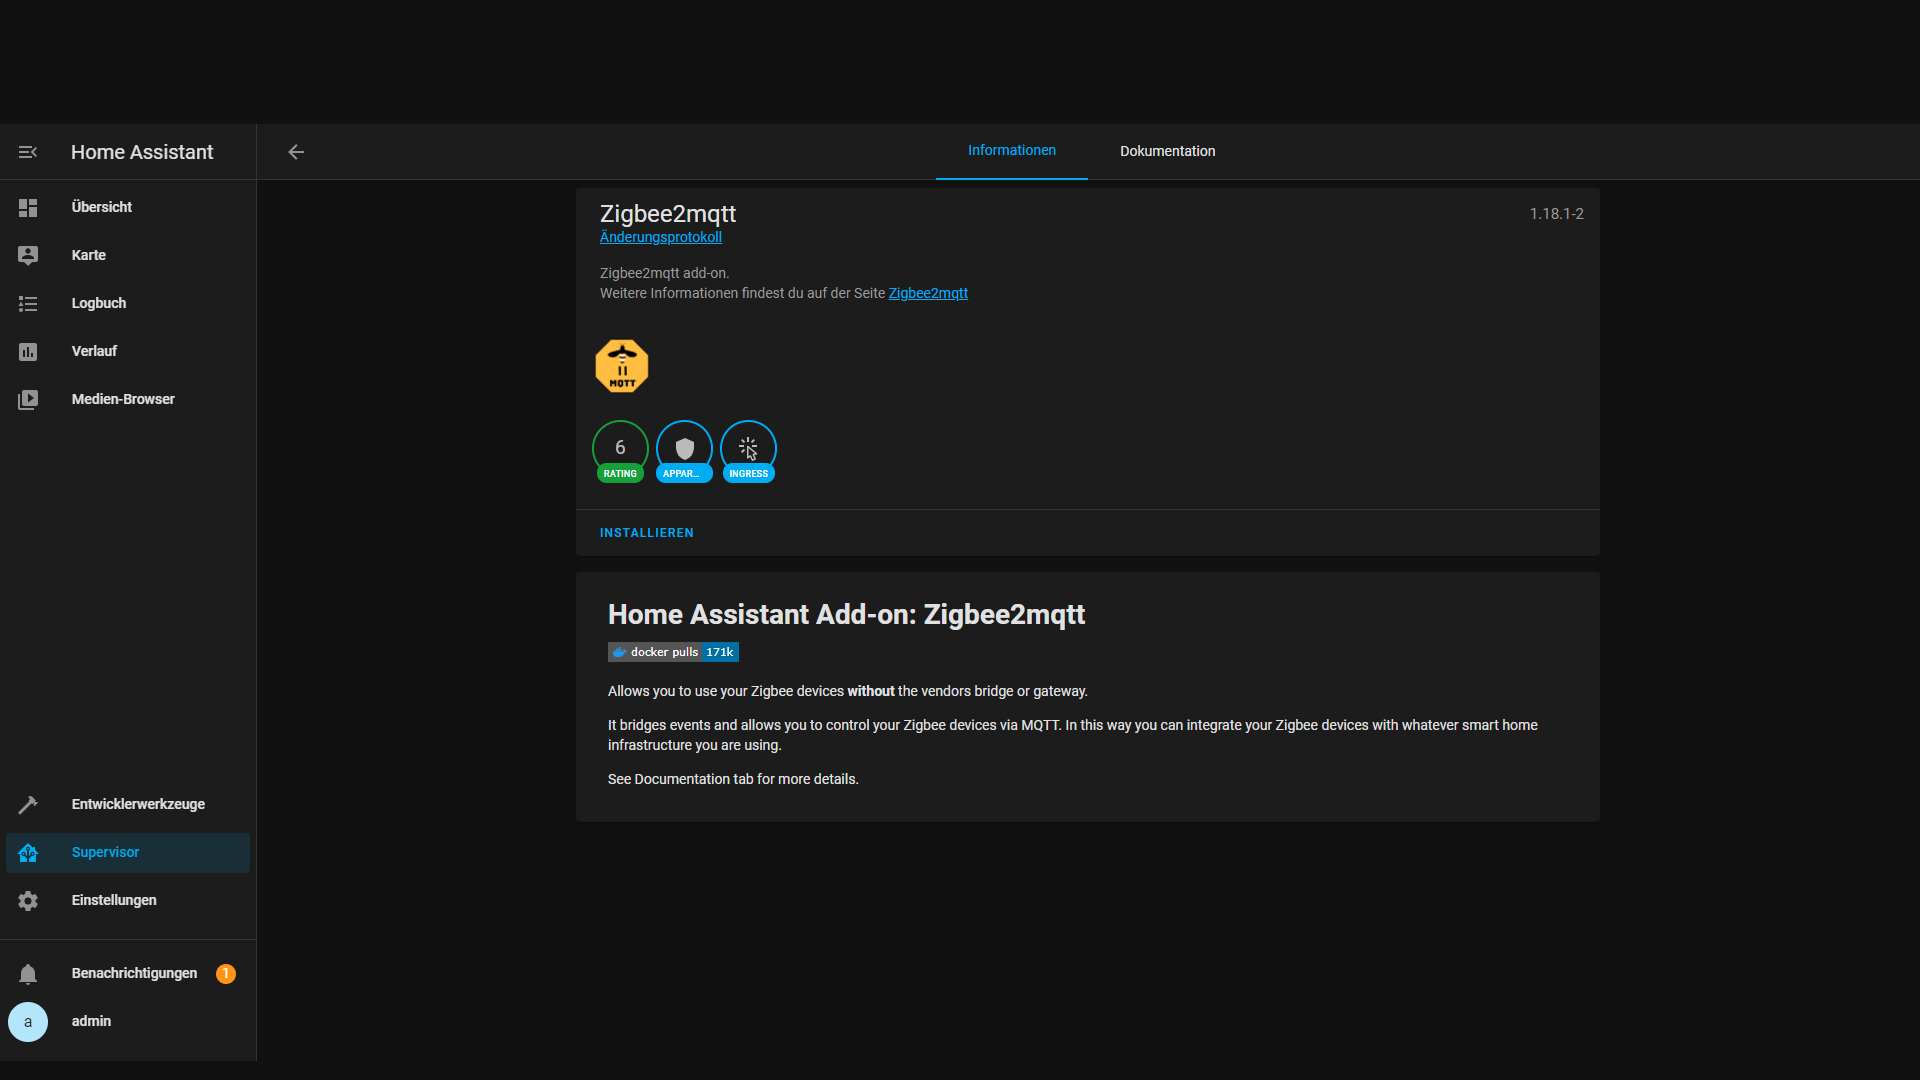
\includegraphics[width=1\textwidth]{img/HA20.png}
        \caption{Zigbee2MQTT add-on seite }
        \label{fig:ha16}
    \end{subfigure}
    \begin{subfigure}{.5\linewidth}
        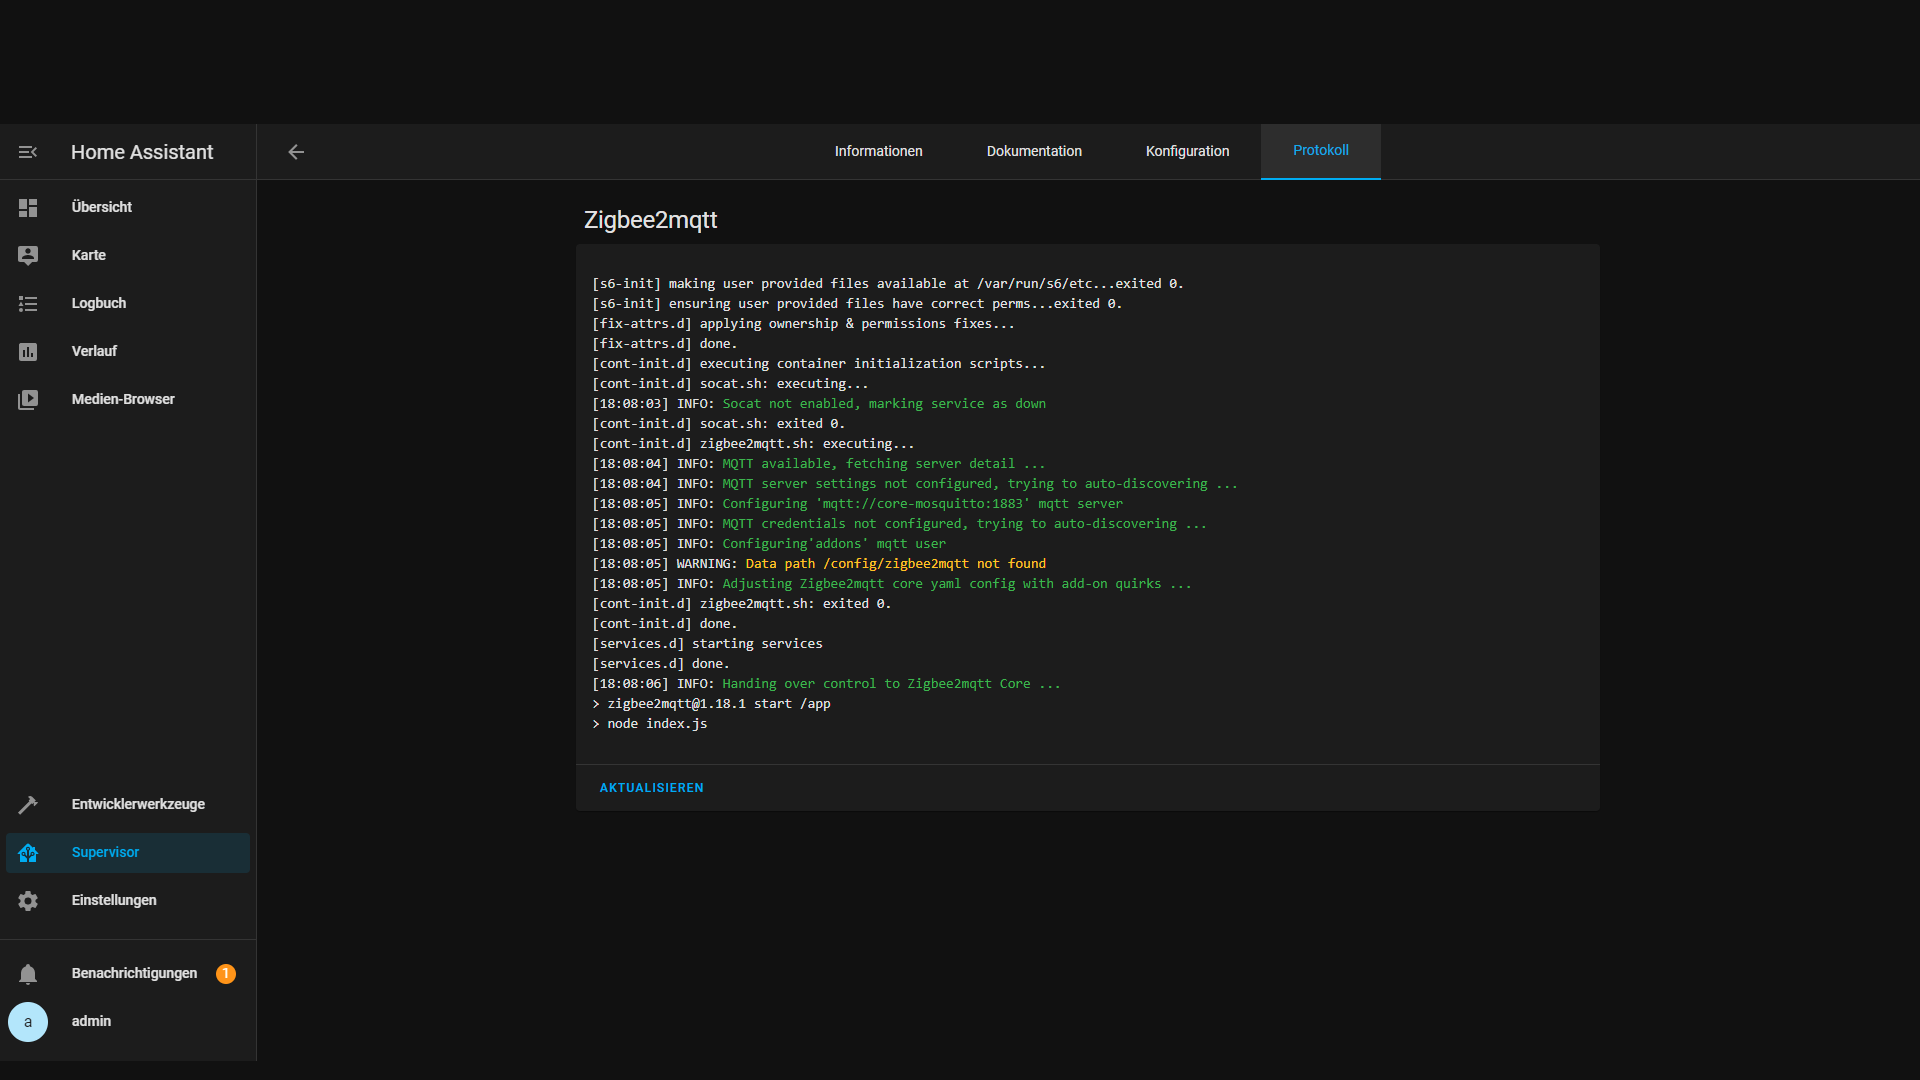
\includegraphics[width=1\textwidth]{img/HA22.png}
        \caption{Configuration.yaml}
        \label{fig:ha18}
    \end{subfigure}
    \begin{subfigure}{.5\linewidth}
        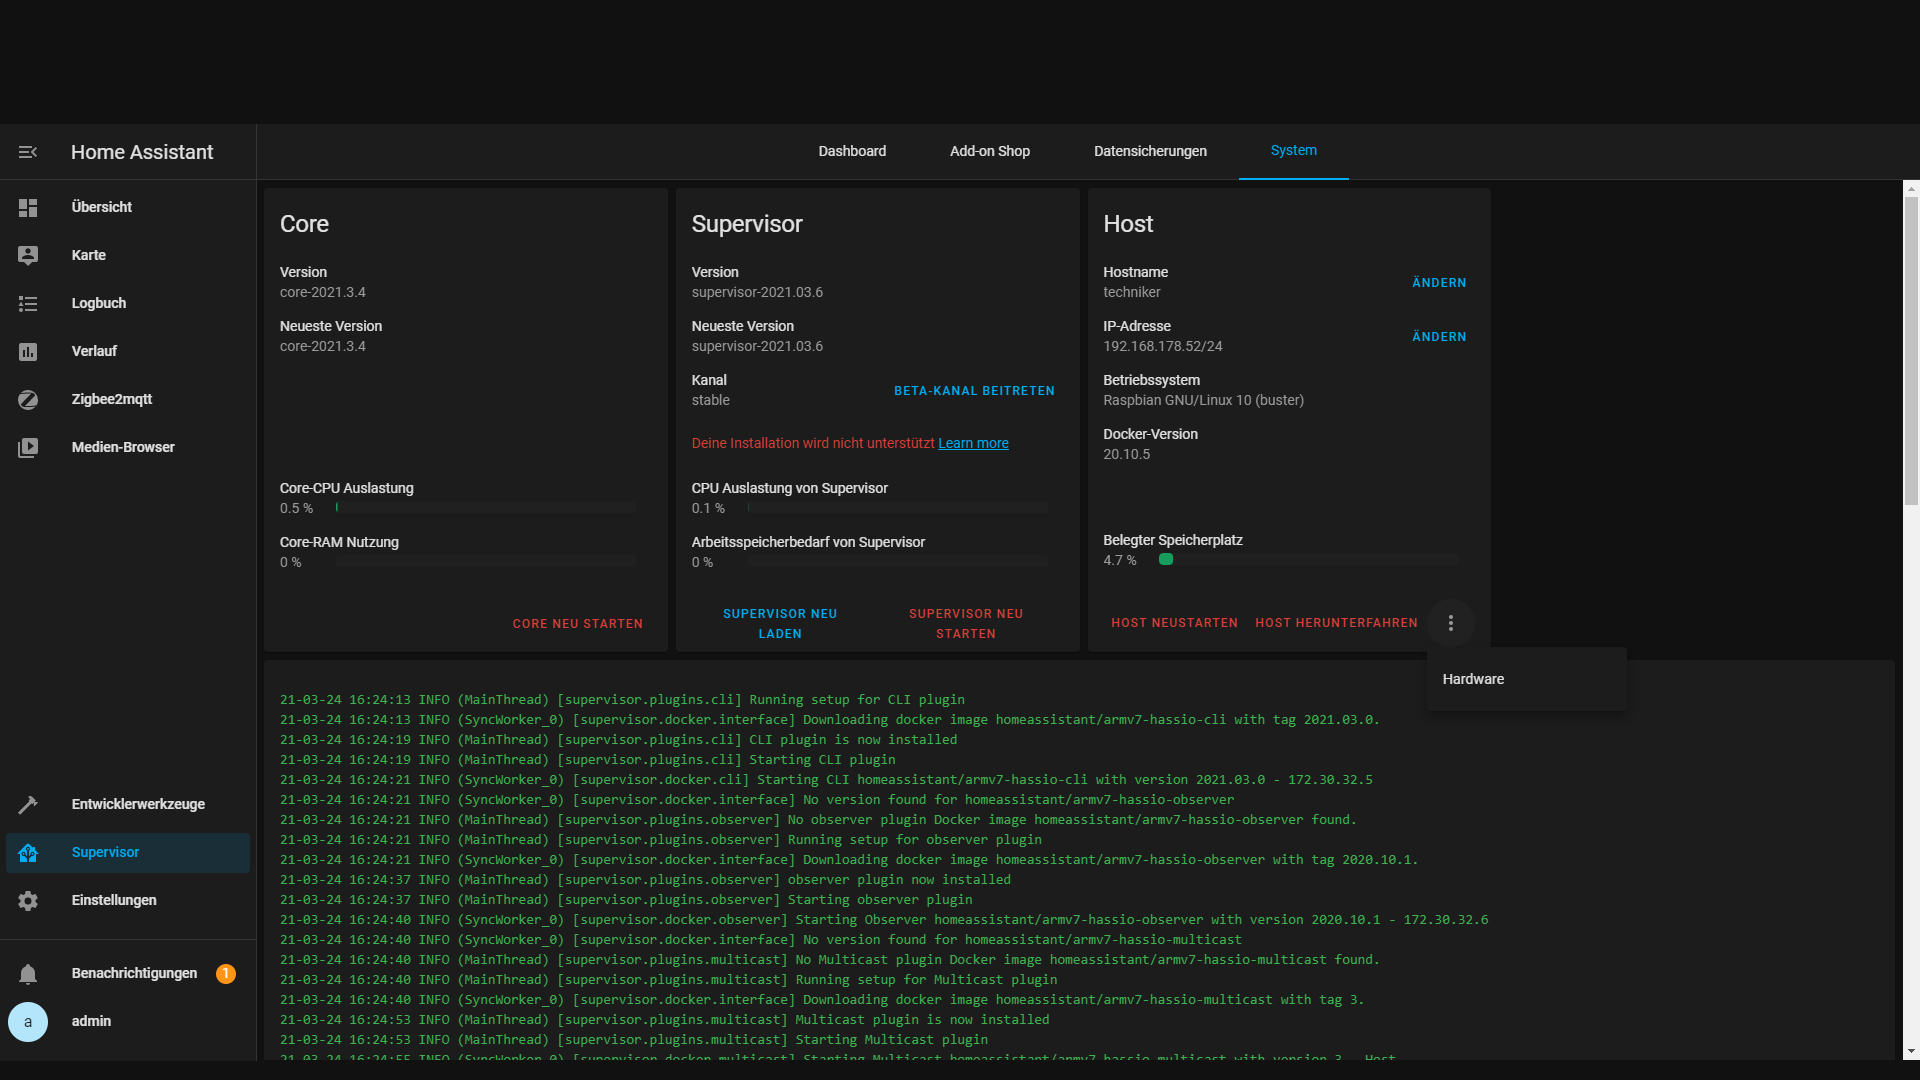
\includegraphics[width=1\textwidth]{img/HA23.png}
        \caption{Supervisor Systeminformationen}
        \label{fig:ha19}
    \end{subfigure}
    \begin{subfigure}{.5\linewidth}
        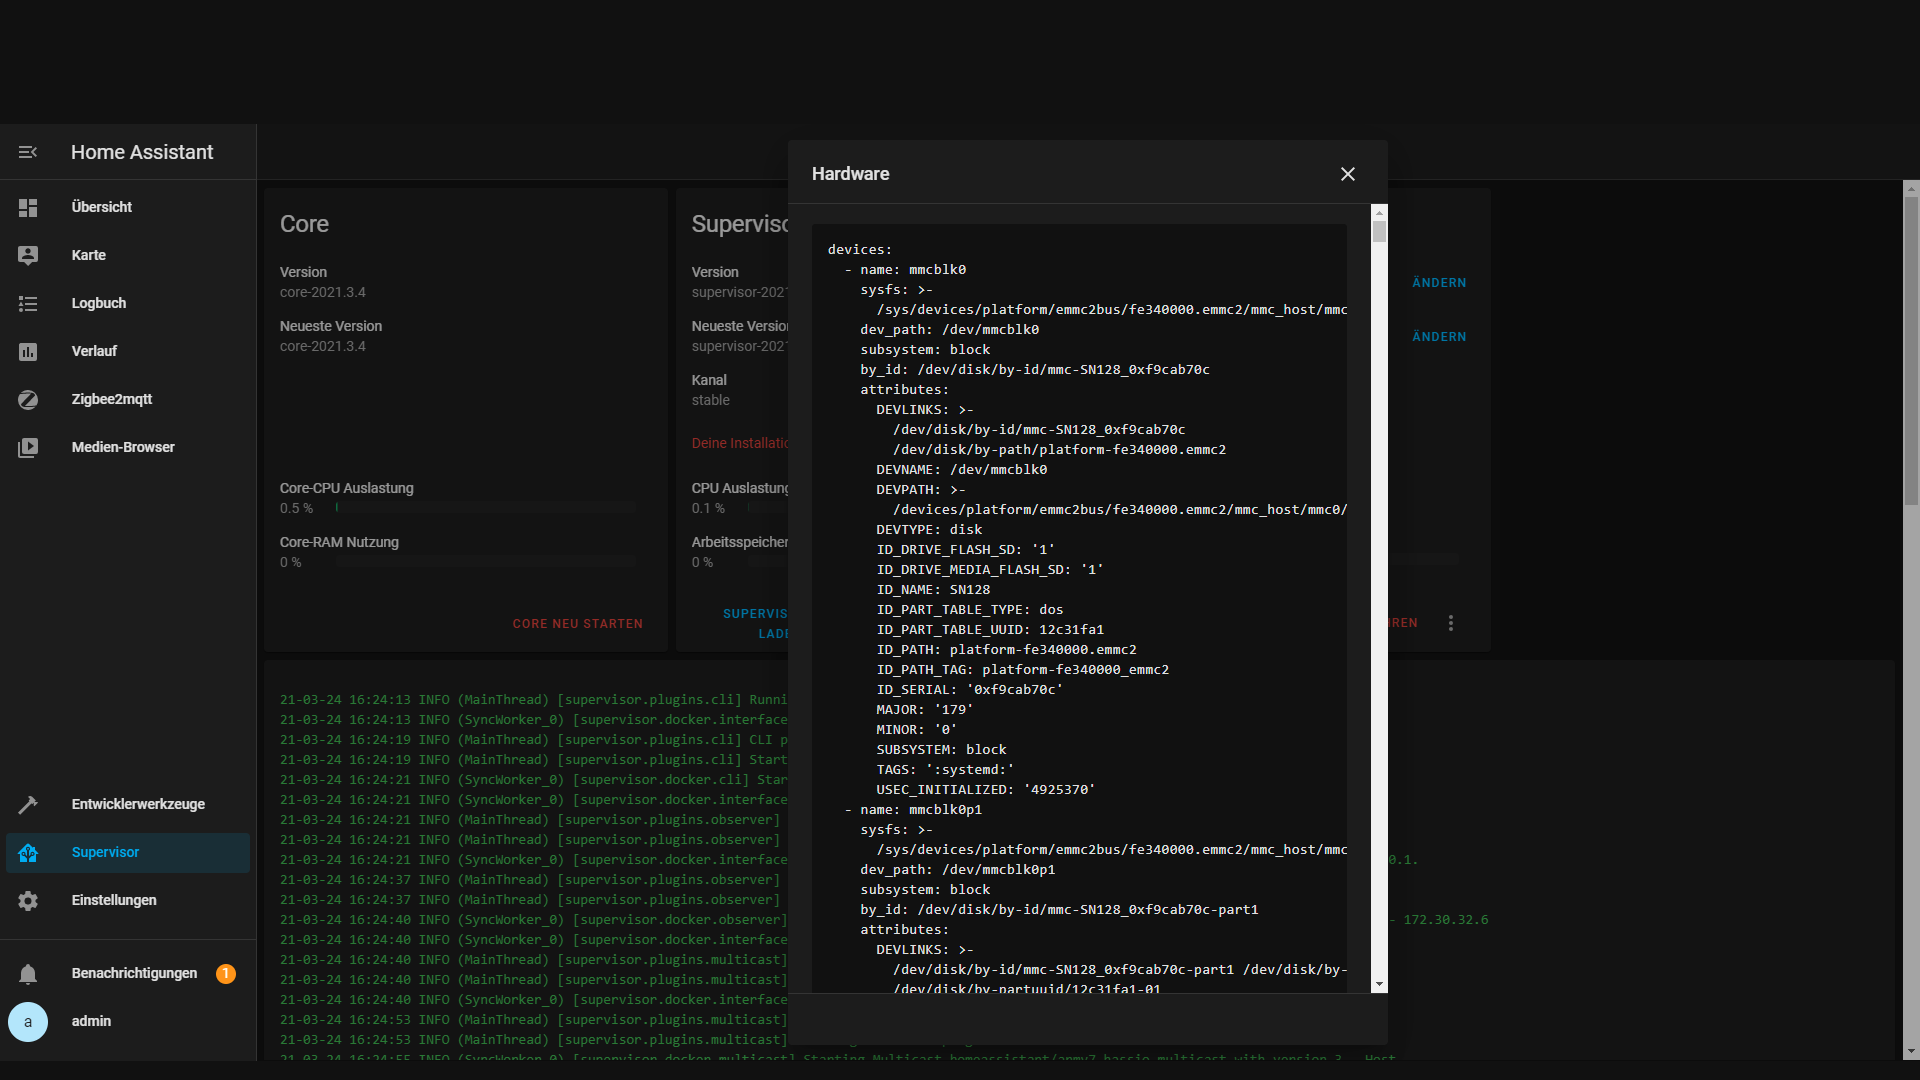
\includegraphics[width=1\textwidth]{img/HA24.png}
        \caption{Auflistung der Hardware}
        \label{fig:ha20}
    \end{subfigure}
    \begin{subfigure}{.5\linewidth}
        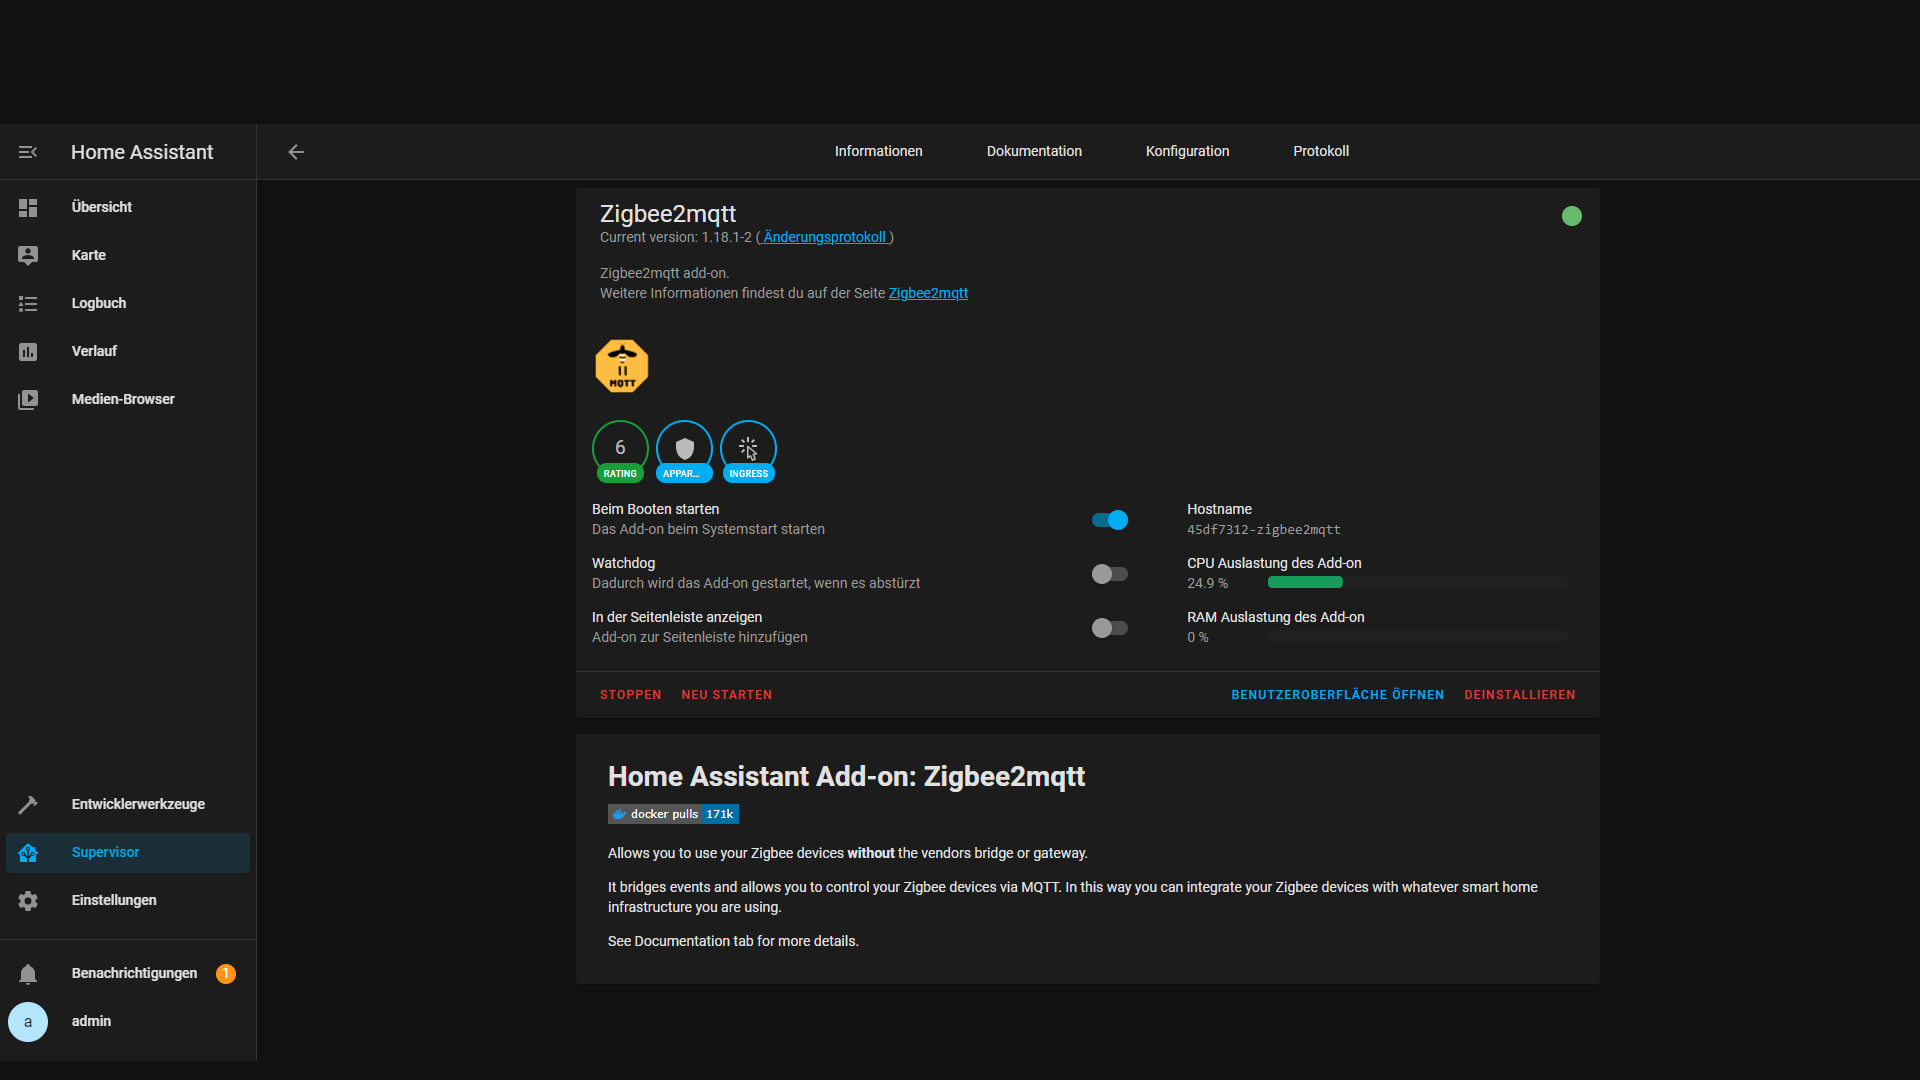
\includegraphics[width=1\textwidth]{img/HA21.png}
        \caption{Aktiviertes Zigbee2MQTT add-on}
        \label{fig:ha17}
    \end{subfigure}
\end{figure}

